\documentclass[10pt]{exam}
\usepackage[phy]{template-for-exam}
\usepackage{graphicx}

\title{E-Learning 11/7/2023 - Projectile Motion PhET Lab}
\author{Rohrbach}
\date{\today}

\begin{document}
\maketitle

\noindent
Go to Schoology and click the link to {\bf ``E-Learning: Projectile Motion PhET Simulation''}.  When the page loads, click the play button.

\begin{itemize}
  \item Go to the ``Intro'' tab.
  \item Drag the cannon to the ground (altitude of 0 m)	and make sure to check the two boxes under Velocity Vectors.
  
  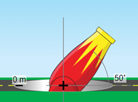
\includegraphics{cannon.png} 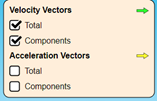
\includegraphics{checkboxes.png}

  \item I will collect this page when you return to class.
\end{itemize}







\begin{questions}
  \question
    Describe the shape of the trajectory made by the projectile.\vs

  \question
    Look back at your notes from last time.  What is meant by the terms $x$-component and $y$-component?  Label on the picture below which one is which.

    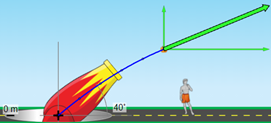
\includegraphics{xy.png}

  \question
    When you fire the cannon, what happens to the x- and y- components of the vector over time? \vs
    
    
  \question
    How does the combination of x- and y- motion give a curved path?  If you need to check the reading from last class to help you, a link is available on Schoology.\vs


  \pagebreak
    
  \question
    On the simulation, increase and decrease the initial speed. How are the range (that is, how far across the ground) and height (that is how far in the air) affected by changing the initial speed? Why do you think this is? \vs
    
  \question
    Change from a pumpkin to a tank shell.  The mass of the tank shell is much larger.  

    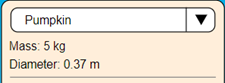
\includegraphics{pumpkin.png} 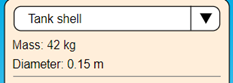
\includegraphics{tankshell.png}
      
    What happens to the trajectory when you use this larger mass?  Why does this make sense? \vs[2]
    
   \question
    Now change the angle.
    
    \begin{parts}
      \part Which angle has the tallest height? \vs
      \part Which angle has the longest range? \vs
      \part Why do you think these angles make sense? \vs
    \end{parts}
    
    \question 
      Can you figure out pairs of angles that give the same range?  Why do you think they give the same range?  Can you notice a pattern? 

      \vspace{1em}
      \fillin[][3em]$^\circ$ and \fillin[][3em]$^\circ$
      
      \vspace{1em}
      \fillin[][3em]$^\circ$ and \fillin[][3em]$^\circ$

      \vspace{1em}
      \fillin[][3em]$^\circ$ and \fillin[][3em]$^\circ$

\end{questions}





\end{document}